\section{Lifted Disjoint Paths}
\label{sec:lifted-disjoint-paths}

The lifted disjoint paths problem is an extension of the node-disjoint paths problem by additional lifted edges that represent connectivity given by the disjoint paths.
They allow to express long-range connectivity priors.

\begin{definition}[Flow Network and Lifted Graph]
Consider two directed acyclic graphs $G = (V, E)$ and $G' = (V',E')$ where $V' =V\backslash \{s,t\}$.
The graph $G=(V,E)$ represents the flow network and we denote by $G'$ the lifted graph.
The two special nodes $s$ and $t$ of $G$ denote source and sink node respectively.
\end{definition}

\begin{definition}[Paths]
We define the set of paths starting at $v$ and ending in $w$ as
\begin{equation}
vw\mhyphen\text{paths}(G) = \{
(v_1v_2,\ldots,v_{l-1}v_l) : \begin{array}{c} v_i v_{i+1} \in E \\ v_1 = v, v_l = w \end{array}
 \}
\end{equation}
For a $vw\mhyphen\text{path}$ $P$ we denote its edge set as $P_E$ and its node
set as $P_V$. 
\end{definition}

\begin{definition}[Lifted Edges]
Given an indicator vector $y \in \{0,1\}^E$ of a node-disjoint set of paths and a lifted edge $e \in E'$ its indicator variable $y'_e \in \{0,1\}$ is defined as
\begin{equation}
\label{eq:lifted-disjoint-paths-lifted-edge}
y'_e \Leftrightarrow \exists P \in vw\mhyphen\text{paths}(G) \text{ s.t. } \forall ij \in P_E : y_{ij} = 1\,.
\end{equation}
\end{definition}

\begin{definition}[Lifted Disjoint Paths Problem]
Given edge costs $c \in \R^E$, node cost $\omega \in \R^V$ for the flow network $G$ and edge costs $c' \in \R^{E'}$ for the lifted graph $G'$ we define the lifted disjoint paths problem as
\begin{equation}
\label{eq:lifted-disjoint-paths}
\begin{array}{cl}
\min\limits_{\substack{y \in \{0,1\}^E, y' \in \{0,1\}^{E'} \\ x \in \{0,1\}^V }} 
&
\la c, y \ra + \la c', y' \ra + \la \omega, x \ra \\
\text{s.t.}
& y \text{ node-disjoint } s,t-\text{flow in } G \\
& x \text{ flow through nodes of } G \\
& y,y' \text{ feasible according to~\eqref{eq:lifted-disjoint-paths-lifted-edge}}\,.
\end{array}
\end{equation}
\end{definition}

An ILP formulation of~\eqref{eq:lifted-disjoint-paths} is given in~\cite{hornakova2020lifted}.
For an illustration of the lifted disjoint paths problem see Figure~\ref{fig:LDP}.

%\begin{figure}[H]
%\centering
%\includestandalone[width=0.8\columnwidth]{figures/lifted-disjoint-paths}
%\caption{
%Illustration of a lifted disjoint paths problem on flow network (black edges) and lifted graph (blue edges).
%Active edges $y,y' = 1$ are solid while inactive edges $y,y' = 0$ are dashed.
%}
%\label{fig:lifted-disjoint-paths}
%\end{figure}

\begin{figure}
	\centering
	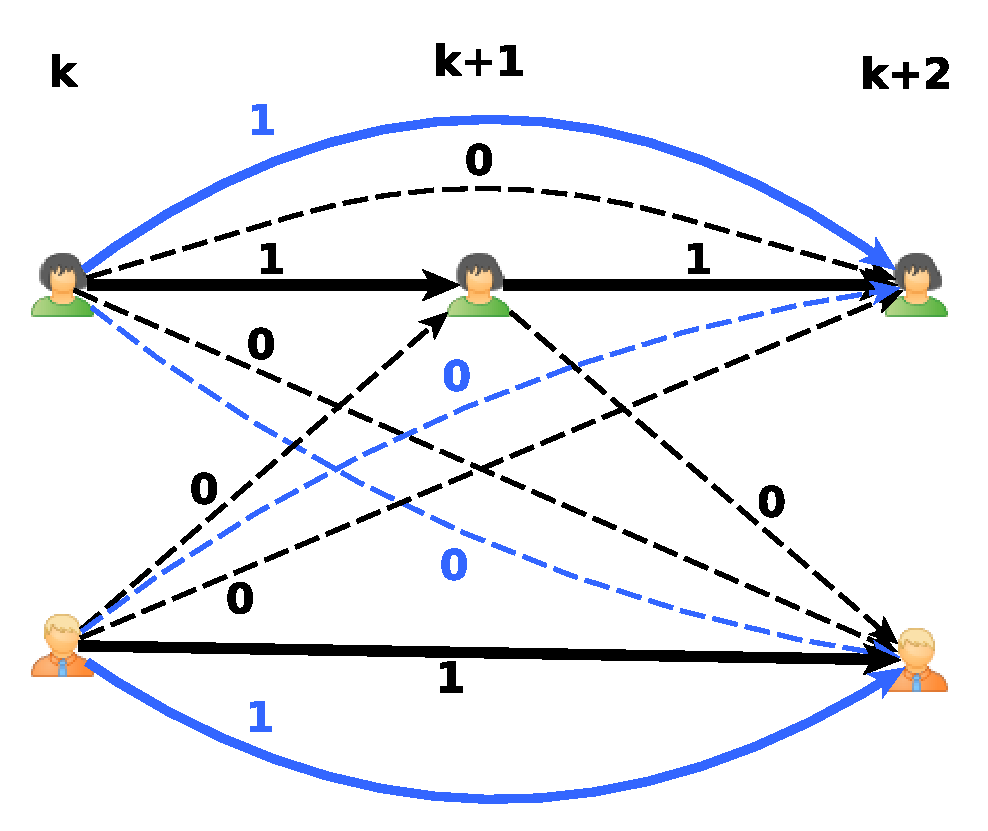
\includegraphics[width=0.9\columnwidth]{images/illustrationLDP}
	\caption{Illustration of a lifted disjoint paths problem on flow network (black edges) and lifted graph (blue edges).
		Active edges $y,y' = 1$ are solid while inactive edges $y,y' = 0$ are dashed.}
	\label{fig:LDP}	
\end{figure}


\subsection{File Format}
File defining costs between pairs of nodes. Some of the pairs are selected to create flow edges, some of them are selected to create lifted edges according to the strategy for graph creation given by solver parameters. Note that lifted and flow edges can overlap. 
\begin{fileformat}
	(*$|V'|$*)
	(*$v_1$*),(*$w_1$*),(*$c_1$*)
	.
	.
	.
	(*$v_m$*),(*$w_m$*),(*$c_m$*) 
\end{fileformat}
File defining which graph nodes belong to which time frames. Time frames are numbered from $1$ to $T$ (maximal time frame). Nodes are numbered from $0$ to $|V'|-1$. $V_i$ denotes nodes in time frame $i$.
\begin{fileformat}
	(*$1$*) (*$0$*)
	(*$1$*) (*$1$*)
	.
	.
	.
	(*$1$*) (*$|V_1|-1$*)
	(*$2$*) (*$|V_1|$*)
	.
	.
	.
	(*$2$*) (*$|V_1|+|V_2|-1$*)
	.
	.
	.
	(*$T$*) (*$|V'|-1$*)
\end{fileformat}
File with solver parameters.
\begin{fileformat}
	[SOLVER]
	FIRST_PARAMETER_NAME=value1
	SECOND_PARAMETER_NAME=value2
	.
	.
	.
\end{fileformat}

\subsection{Datasets}

\subsection{Algorithms}
\begin{description}
    \item[ILP Solver~\cite{hornakova2020lifted}:] Cutting planes for ILP solvers together with a two-stage procedure for computing tracklets first.
    \item[Message Passing Solver~\cite{hornakova2021making}:] Decompose the full problem into combinatorially solved subproblems and link them together with Lagrange multipliers updated by block coordinate ascent.
\end{description}
